\documentclass[11pt,DIV=10,final]{scrreprt} %11pt legt die generelle Schriftgrösse fest, DIV die Seitenaufteilung (Seitenränder): lieber viele Seiten als zu kleine Seitenränder!
%ändert man "final" zu "draft", werden speicheraufwändige Elemente nicht eingebunden: Genau das richtige für die Plagiatsprüfung

%*************** Paket-Einbindungen: ******************
\usepackage[utf8]{inputenc} %damit man auch Umlaute eingeben kann
\usepackage[bitstream-charter]{mathdesign} % Charter als Standardschriftart
\usepackage[scaled=.82]{DejaVuSansMono} % DejaVuSansMono als Code-Schriftart
\usepackage[T1]{fontenc} %damit Umlaute bei einer pdf-Suche auch erkannt werden
\usepackage{amsfonts,amsmath} %Verwendung von Mathematik-Schriftarten
\usepackage{graphicx} %für Grafiken der Formate jpg, png, pdf
\usepackage{float} % um Abbildung wirklich genau dort zu platzieren
\usepackage{url} %für die gute Darstellung von Internet-Links
\usepackage[ngerman]{babel} %deutsches Sprachpaket
\usepackage[round]{natbib} %für vereinfachtes Zitieren/Querverweise
\usepackage{listings} % für Quelltext mit Syntax-Highlighting
\usepackage{tikz} %für tikz-Grafiken
\usetikzlibrary{graphs} %für Graphen (also auch Neuronale Netze) in tikz

%************** Zusätzliche Einstellungen und eigene Befehle:  **********
\setkomafont{sectioning}{\rmfamily\bfseries\boldmath} % verwende für die Titel die selbe Schriftart wie für Fliesstext

\tikzset{>=stealth} % schönere Pfeilspitzen in TikZ-Grafiken

\lstnewenvironment{cppcode}[1][] % für abgesetzten C++ Code
{\lstset{
	language=C++,
	%backgroundcolor=\color[HTML]{E8F2F2},
	basicstyle=\small\ttfamily,
	keywordstyle=\color{blue},
	commentstyle=\color{brown}, 
	numbers=left,
	%numberstyle=\tiny,
	%frame=leftline,
	%xleftmargin=.04\textwidth,
	inputencoding=utf8,
	extendedchars=true,
	literate={ä}{{\"a}}1 {à}{{\`a}}1 {ö}{{\"o}}1 {ü}{{\"u}}1 {è}{{\`e}}1 {é}{{\'e}}1,
	#1}}{}
	
\providecommand{\cppinline}{\lstinline[language=C++,basicstyle=\ttfamily,keywordstyle=\color{blue},commentstyle=\color{brown}, literate={ä}{{\"a}}1 {à}{{\`a}}1 {ö}{{\"o}}1 {ü}{{\"u}}1 {è}{{\`e}}1 {é}{{\'e}}1]} % für Inline-C++ Code

\begin{document}

\begin{titlepage}
\mbox{}\vspace{0.1\textheight}
\begin{center}
\textbf{\Huge Mein Titel}\\[3ex]
Gian Laager\\
\today
\vspace{0.05\textheight}
\begin{center}
	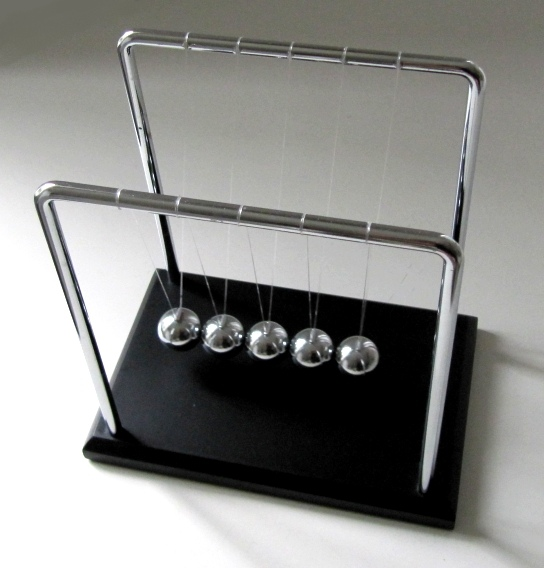
\includegraphics[width=.7\textwidth]{titelbild.jpg}
\end{center}
\vspace{0.05\textheight}
Maturaarbeit\\
Kantonsschule Glarus\\
Betreuer: Linus Romer\\
Referent: Beat Temperli
\end{center}
\end{titlepage}

\pagenumbering{roman}   % i, ii, iii, iv, ...

\chapter*{Dank}
Mein ausserordentlicher Dank gilt Fritz Muster für das Korrekturlesen. Ebenso danke ich Heiri Müller und Otto Normalverbraucher für ihre hilfreichen Korrespondenzen mit mir.

\tableofcontents %Inhaltsverzeichnis

\chapter{Einleitung}\pagenumbering{arabic}  % 1, 2, 3, 4, ...
Bla

Fragestellung
\begin{itemize}
	\item aaa
	\item aaa
\end{itemize}

\chapter{Präliminarien}
$\hbar$

Allgemein ist ``The Not So Short Introduction to LaTeX'' sehr empfehlenswert als Referenz für \LaTeX. Kurztipps zum Formelsatz: Kleinere Formeln wie $c^2=a^2+b^2$ können problemlos direkt im Text platziert werden. Grössere Formeln sollten jedoch abgesetzt präsentiert werden:
\[
	T\approx 2\pi\sqrt{\frac{J_s+ms^2}{mgs}}
\]
Wenn sie extrem wichtig sind, kann man sie auch umrahmen:
\[
	\boxed{T\approx 2\pi\sqrt{\frac{J_s+ms^2}{mgs}}}
\]

Dieses Theorem \citep[S.~117]{alexandrov55} wird oft verwendet.

%Dieser Text steht in Anlehnung an \citet{alexandrov55}. 

%Dieser Text steht in Anlehnung an \citet[Kap.~2]{alexandrov55}. 

%Dieses Theorem \citep{alexandrov55} wird oft verwendet. 

%Dieses Theorem \citep[Kap.~2]{alexandrov55} wird oft verwendet. 

%Dieses Theorem \citep[siehe][]{alexandrov55} wird oft verwendet. 

%Dieses Theorem \citep[siehe][Kap.~2]{alexandrov55} wird oft verwendet. 

Mehrere Zeilen (oder Gleichungssysteme) löst man mit der align-Umgebung:
\begin{align*}
	a^2+b^2 &= c^2\\
	d &= \frac{a}{c}
\end{align*}
Falls man möchte, kann man die Formeln auch nummerieren lassen:
\begin{align}
	a^2+b^2 &= c^2\\
	d &= \frac{a}{c}
\end{align}
Was zu dieser Referenz gehört, steht in der literatur.bib. Wenn man die Referenzen ändert, sollte man zwischendurch BibTeX über das Hauptdokument laufen lassen. Falls irgendetwas einfach nicht mehr klappen sollte, muss man vielleicht die Hilfsdateien entfernen (Datei/Hilfsdateien entfernen) und nochmals pdflatex, bibtex, pdflatex darüber laufen lassen.

Noch ein paar weitere Referenzen zu einem Artikel \citep{kleinerleeb97}, zu einem Wikipedia-Artikel \citep{wikipediapendel} und einem Artikel mit bekanntem Author \citep{knuth}.

Was viele beim Start mit \LaTeX{} verpassen, sind Querverweise innerhalb des Dokuments, also nicht zur Literatur. Die löst man mit label und ref:

\section{Abschnitt, auf den ich Bezug nehmen will}
\label{sec:meinspecialabschnitt}
Hier nehme ich Bezug auf den Abschnitt~\ref{sec:meinspecialabschnitt}. Der Trick dabei ist es, dass man das label direkt nach dem einleitenden Befehl verwendet. Das funktioniert dann z.~B. auch für Abbildungen. Bilder können theoretisch textumflossen eingebunden werden, layouterisch sauberer ist jedoch in einer Arbeit oft, dass man Bilder abgesetzt einbindet.
\begin{figure}[H]
	\begin{center}
		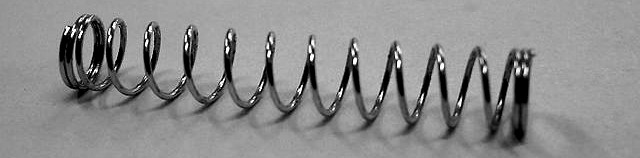
\includegraphics[width=.8\textwidth]{kugelschreiberfeder.jpg}
		\caption{Eine Kugelschreiberfeder \citep{wikipediapendel}.}
		\label{fig:kugelschreiberfeder}
	\end{center}
\end{figure}
Die «figure»-Umgebung könnte man auch weglassen, aber gemäss Reglement muss jede Abbildung eine Bildunterschrift haben und für das braucht man dann «figure». Hier nehme ich Bezug auf die Abbildung~\ref{fig:kugelschreiberfeder}. Die figure-Umgebung kann auch selbständig wählen, wo ein Bild gesetzt werden soll. Dann lässt man die Option [H] (für Here) einfach weg.

Hier noch ein Beispiel mit \emph{TikZ}:
\begin{figure}[H]
	\begin{center}
		\begin{tikzpicture}
			\graph {a -> {b -> e -> {f,g}, c -> h -> g,d -> h}; i -> {b,d}; };
		\end{tikzpicture}
		\caption{Graph des Neuronalen Netzwerks.}
		\label{fig:neuronalesnetzwerk}
	\end{center}
\end{figure}

\section{Künstliche Intelligenz}
\section{Maschinelles Lernen}
\subsection{Unterschiedliche Algorithmen des Maschinellen Lernens}
\section{Genetische Algorithmen}
\subsection{Biologie der Genetischen Algorithmen}
\section{Neuronale Netzwerke}
\subsection{Biologie der Neuronalen Netzwerken}
\section{Neuroevolution}
\subsection{Vorteile der Neuroevolution}
\subsection{Nachteile der Neuroevolution}
\chapter{Methoden}
\section{Programmiersprache}
\section{Algorithmus}
Inline-Codes wie \cppinline{predict(std::vector<double> inputs)} sind für Quelltext-Ausschnitte gedacht, die kürzer als eine Zeile sind (meistens für Header von Funktionen verwendet). Für mehrere Quelltext-Zeilen verwendet man:
\begin{cppcode}
#include "NeuralNetwork.h"
#include "Profiler.h"

void nn::NeuralNetwork::calculateNeuron(neuron::Neuron* neuron)
{
    neuron->calculate();
}

std::vector<double> nn::NeuralNetwork::predict(std::vector<double> inputs)
{
    // check if the inputs have the right length
    if (inputs.size() != this->inputLayer->size)
    {
        std::cout << "Input vector has to be the same size as the input Layer" << std::endl;
        throw ("Input vector has to be the same size as the input Layer");
    }

    // reset the cache on the neurons 
    for (neuron::Neuron* c_neuron: *this->neurons)
    {
        c_neuron->rewriteCache = true;
    }

    // set the values on the input neurons
    for (int i = 0; i < this->inputLayer->size; i++)
    {
        this->inputLayer->neurons.at(i)->value = inputs.at(i);
    }

    // create the result vector
    std::vector<double> result = std::vector<double>();
    result.reserve(this->previousLayerSize);

    // feedforward
    for (int i = 0; i < this->outputLayer->neurons.size(); i++)
    {
        neuron::Neuron* c_neuron = this->outputLayer->neurons.at(i);
        result.push_back(c_neuron->recursiveCalculate());
    }

    return result;
}
\end{cppcode}

\section{Anwendungsbeispiel}
\chapter{Ergebnisse}
\section{Programmstruktur}
\section{Messwerte}
\chapter{Diskussion}
\section{Programm}
\subsection{Schwierigkeiten}
\subsection{Verbesserungsmöglichkeiten}
\subsection{Performance}
\chapter{Fazit}



%
\begin{appendix} %Anhang falls nötig
%
\chapter{Quelltext der Programme}
%
bla
\chapter{Detaillierte Berechnungen}
%
bla
%
\end{appendix}
%
\chapter*{Bildquellen}
%
Wo nicht anders angegeben, sind die Bilder aus dieser Arbeit selbst erstellt worden. Das Titelbild stammt aus \citet{wikipediapendel}.
%
\bibliographystyle{plainnatromer}
\bibliography{literatur}
%
\chapter*{Selbständigkeitserklärung}
%
Hiermit bestätige ich, Hans Muster, meine Maturaarbeit selbständig verfasst und alle Quellen angegeben zu haben.\\\newline
Ich nehme zur Kenntnis, dass meine Arbeit zur Überprüfung der korrekten und vollständigen Angabe der Quellen mit Hilfe einer Software (Plagiaterkennungstool) geprüft wird. Zu meinem eigenen Schutz wird die Software auch dazu verwendet, später eingereichte Arbeiten mit meiner Arbeit elektronisch zu vergleichen und damit Abschriften und eine Verletzung meines Urheberrechts zu verhindern. Falls Verdacht besteht, dass mein Urheberrecht verletzt wurde, erkläre ich mich damit einverstanden, dass die Schulleitung meine Arbeit zu Prüfzwecken herausgibt.\\\newline
Ort\hspace{4cm} Datum\hspace{4cm}  Unterschrift
%
\end{document}

